\input{header}

\AtBeginSubsection[]
{
	\begin{frame}<beamer>
		\frametitle{Outline}
		\tableofcontents[current,currentsubsection]
	\end{frame}
}

\begin{document}

\begin{frame}[allowframebreaks] \frametitle{Complexity}
  \begin{itemize}
\item Decidable $\rightarrow$ computationally solvable
\item may Not solvable in practice

\end{itemize}\end{frame} \begin{frame}[allowframebreaks] \frametitle{Example}
  \begin{itemize}
\item $A=\{0^k 1^k\mid k \geq 0\}$

\# steps by a TM ? (1-tape)
\item Remember the procedure
  \begin{enumerate}
  \item check $0^? 1^{??}$
  \item repeat until no 0 or 1

scan, cross off single 0 and 1
\item if 0 or 1 remains, reject

otherwise, accept

  \end{enumerate}
\item How much time ?

\# steps
\end{itemize}\end{frame} \begin{frame}[allowframebreaks] \frametitle{Analysis}
  \begin{itemize}
\item worst-case analysis

longest time for all inputs

\item average-case analysis
\item $f: N \rightarrow N$

$N$: natural number

$n$: length of input

\end{itemize}\end{frame} \begin{frame}[allowframebreaks] \frametitle{Big-O}
  \begin{itemize}
\item $f(n)=6n^3 + 5$

$n \rightarrow \infty, 6n^3 + 5 \approx 6n^3$
\item $O(f(n))=O(n^3)$

How about 6 ?

$6n^3$ vs. $n^3$

$6n^3$ vs. $n^4$

only things involved with $n$ important
\end{itemize}\end{frame} \begin{frame}[allowframebreaks] \frametitle{Definition}
  \begin{itemize}
\item $f(n)=O(g(n))$ if 

  \begin{equation*}
    \exists c, n_0, \forall n \geq n_0,
f(n) \leq c g(n).
  \end{equation*}
\end{itemize}\end{frame} \begin{frame}[allowframebreaks] \frametitle{Example}
    \begin{itemize}
\item $f(n) = 6n^3 + 5$

$6n^3 + 5 \leq 7n^3$ after $n \geq 2$

$c=7$

so $f(n) = O(n^3)$
\item $f(n)=O(n^4)$ as 

$6n^3+5 \leq 7n^4$, after $n \geq 2$
\item But $f(n) \neq O(n^2)$

$6n^3+5 \leq c n^2$, choose large $n$, $n^3 > cn^2$

\end{itemize}\end{frame} \begin{frame}[allowframebreaks] \frametitle{Example 7.4}
  \begin{itemize}
\item $f(n)=3n \log_2 n + 5n \log_2 \log_2 n
$

$f(n) = O(n\log n)$

$\log_2 \log_2 n \leq \log_2 n$
from $\log_2 n \leq n$

$f(n) \leq 8n \log_2 n = 8n\log_2 b\log_b n$

$\log_2 n / \log_2 b= \log_b n$

(can be an exercise)

\item $f(n)=O(n\log n)$, not need to write $\log_2 n$
\end{itemize}\end{frame} \begin{frame}[allowframebreaks] \frametitle{Other properties}
  \begin{itemize}
\item $O(n^2) + O(n) = O(n^2)$

$\leq c_1 n^2 + c_2 n $ after $n \geq \max(n_1,n_2)$

$\leq (c_1+c_2) n^2$
\item $2^{O(n)} \equiv \leq 2^{cn}$
\item $O(1): \leq c 1$

$\Rightarrow$ always $\leq$ a constant
\end{itemize}\end{frame} \begin{frame}[allowframebreaks] \frametitle{Small-o}
  \begin{itemize}
\item opposite

$O$: no more than ??

$o$: less than ??
\item Definition 

$f(n)=o(g(n))$ if
  \begin{equation*}
    \lim_{n\rightarrow \infty} \frac{f(n)}{g(n)} = 0.
  \end{equation*}
the definition of this limit ?
\begin{equation*}
  \forall c > 0, \exists N, \forall n \geq N,
\frac{f(n)}{g(n)} < c.
\end{equation*}
\end{itemize}\end{frame} \begin{frame}[allowframebreaks] \frametitle{Example}
  \begin{itemize}
\item $\sqrt{n}= o(n)$
  \begin{equation*}
    \lim_{n \rightarrow \infty} \frac{\sqrt{n}}{n}
=
   \lim_{n \rightarrow \infty} \frac{1}{\sqrt{n}}=0
  \end{equation*}
\item $f(n) 
\neq o(f(n))$
\end{itemize}\end{frame} \begin{frame}[allowframebreaks] \frametitle{Analyzing: $A=\{0^k 1^k\mid k \geq 0\}$}
    \begin{itemize}
\item check 0...0 1...1: $O(n)$

move back $O(n)$
\item cross off each 0 and 1: $O(n)$

How many such crosses: $n/2$

$n/2 \times O(n) = O(n^2)$
\item accept or not ?

$O(n)$
\item $O(n) + O(n^2) +O(n) = O(n^2)$
\end{itemize}\end{frame} \begin{frame}[allowframebreaks] \frametitle{Def: Time complexity class}
  \begin{itemize}
\item TIME$(t(n))$

\{ $L\mid L$ language decided by an $O(t(n))$
TM
\}
\item $\{0^k 1^k \mid k \geq 0\} \in \textrm{TIME}(n^2)$

can we make it faster

\end{itemize}\end{frame} \begin{frame}[allowframebreaks] \frametitle{New Algorithm $M_2$}
  \begin{itemize}
\item The procedure
$\underline{0}0
\underline{0}0
\underline{0}
\underline{1}1
\underline{1}1
\underline{1}
$

$\underline{0}0
\underline{1}1
$

$\underline{0}
\underline{1}
$

$\epsilon$

key: total must be even

\item A failed algorithm


$\underline{0}0
\underline{0}0
\underline{1}1
$

$001
$

\item 
Algorithm
\begin{enumerate}
\item check 0...0 1...1
\item repeat if not empty 

total \# 0 \& 1: odd $\Rightarrow$ reject

cross off every other 0 and 1
\item no 0 \& 1 remain, accept
\end{enumerate}
\item If  13 ``0'' $\Rightarrow$
6 ``0'' $\Rightarrow$
3 ``0'' $\Rightarrow$
1 ``0'' 

$1+\log_2 n$ iterations

each iter: $O(n)$ operations

$O(n \log n)$

\item $\{0^k 1^k\mid k \geq 0\} \in TIME(n \log n)$

can we do better ? no

Any language decided in $o(n\log n)$
on a single-tape TM $\Rightarrow$ regular
(not proved here)

$\{0^k1^k \mid k \geq 0\}$ is not

\end{itemize}\end{frame} \begin{frame}[allowframebreaks] \frametitle{Using two-tape TM}
  \begin{itemize}
\item $O(n)$  time
\item Procedure 
  \begin{enumerate}
  \item check 0...0 1...1

  \item copy 0 to 2nd tape

find the first 1
\item sequentially cut 1 and 0

if no ``0'' reject
\item if ``1'' left, reject

otherwise, accept
  \end{enumerate}

\item Each step $O(n)$

\end{itemize}\end{frame} \begin{frame}[allowframebreaks] \frametitle{Computability theory vs. complexity theory}
    \begin{itemize}
\item Church-Turing thesis

models equivalent
\item ``time complexity'' different
\item differences not that large for similar models

Next theorem shows that 1 and 2 tapes not very different

\end{itemize}\end{frame} \begin{frame}[allowframebreaks] \frametitle{Theorem 7.8}
  \begin{itemize}
  \item
    $O(t(n))$ multi-tape TM

$\Rightarrow \exists$ equivalent 
$O(t(n)^2)$ single-tape TM
\item idea: similar to how we proved their equivalence

Show simulating each step of a multi-TM
takes
$O(t(n))$ on a single

\end{itemize}\end{frame} \begin{frame}[allowframebreaks] \frametitle{Proof of Theorem 7.8}
  \begin{itemize}
\item We only show a rough proof

\item $k$: \# of tapes
\item How to simulate a multi-tape TM ?

Fig 3.14
\item initial: input to 1st tape, $O(n)$
\item Each step: scan to know where heads point to.

scan to update

may have to right shift the tape
\begin{equation*}
  O(t(n))+O(n)
\end{equation*}
\item Each tape of $M$: $O(t(n))$ length:

An $O(t(n))$ multi-tape TM generates
$O(t(n))$ contents in 
$O(t(n))$ time $(O(t(n))\geq n)$.


\item Each step on $S$: $O(t(n))$

$t(n) \geq n$, so $O(t(n)^2)$


\item Key: \# tapes: a constant order

\end{itemize}\end{frame} \begin{frame}[allowframebreaks] \frametitle{Nondeterministic TM}
  \begin{itemize}
\item Remember NTM a decider if all branches halt on all inputs
\item Figure 7.10

\item time complexity:

Definition of time $f(n)$: maximum \# of steps the machine uses on any branch
on any input length $n$

\end{itemize}\end{frame} \begin{frame}[allowframebreaks] \frametitle{Theorem 7.11}
  \begin{itemize}
  \item $t(n) \geq n, O(t(n))$ NTM (single tape)

$\Rightarrow \exists 2^{O(t(n))}$ TM (single tape)
\item Assume $b$: maximal \# of branches in the tree
\item remember: depth-first way simulation
\item total nodes: $O(b^{t(n)})$
\item depth $d$ finished, do $d+1$

tape 3: all possible paths so far

tape 2: original input w, simulate one path, 1 step further
with all possible branches

simulate tape 2: $O(t(n))$

shift tape 3: $O(b^{(t(n))})$

total cost $\leq O(b^{t(n)})$ for each node
\item total time: $O(b^{t(n)}b^{t(n)})$

$=O((b^2)^{t(n)} )
= O(2^{t(n)})$


\item this is by a 3-tape TM
\item Note $(2^{O(t(n))})^2
= 2^{O(2t(n))}
= 2^{O(t(n))}$

\begin{equation*}
  (2^{O(t(n))})^2
\leq (2^{ct(n)})^2
= 2^{2ct(n)} 
= 2^{O(t(n))}
\end{equation*}

\end{itemize}\end{frame} \begin{frame}[allowframebreaks] \frametitle{Polynomial vs. Exponential}
  \begin{itemize}
\item Big difference
\item $n^3: n = 1000 \Rightarrow 10^9$
\item $2^n: n = 1000 \Rightarrow 2^{1000}
=10^{1000\log_{10}2}
\approx
10^{300}
\gg 10^9$

not practical
\item now we focus on the difference between polynomial
and non-polynomial
\end{itemize}\end{frame} \begin{frame}[allowframebreaks] \frametitle{Definition 7.2}
  \begin{itemize}
\item $P$: decidable languages in polynomial time
on a deterministic (single-tape) TM
\begin{equation*}
  P=\cup_k
\text{TIME}(n^k).
\end{equation*}
\item How important this is ?

$P$: ``roughly'' corresponds to problems solvable
on a computer

% \end{itemize}\end{frame} \begin{frame}[allowframebreaks] \frametitle{Examples of P}
% \item Description on pages 236 and 237

% not very important

\end{itemize}\end{frame} \begin{frame}[allowframebreaks] \frametitle{PATH problem}
\begin{eqnarray*}
&&  \text{PATH}
=\{
\langle  G,s,t\rangle \mid \mbox{$G$ is a directed graph}\\
&& \qquad\qquad\qquad
\mbox{s.t. $\exists$ path from $s$ to $t$}\}
\}
\end{eqnarray*}
  \begin{itemize}
  \item Example:

  \begin{center}
    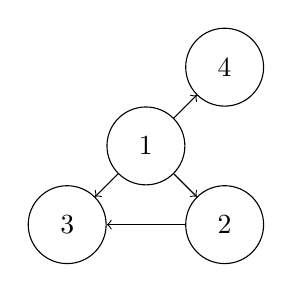
\begin{tikzpicture}
[inner sep=2.5mm]      
\path ( 0,0) node (3) [shape=circle,draw] {3}
( 2,0) node (2) [shape=circle,draw] {2}
( 2,2) node (4) [shape=circle,draw] {4}
( 1,1) node (1) [shape=circle,draw] {1};
\draw [->] (1) -- (2);
\draw [->] (2) -- (3);
\draw [->] (1) -- (3);
\draw [->] (1) -- (4);
\end{tikzpicture}
\end{center}
\item[] There is a path from $s=1$ to $t=3$
\item PATH $\in P$
\item Brute force way

$m$: \# nodes

$|\text{path}|\leq m$

\#paths $\leq m^m$

sequentially check if one has $s$ to $t$

Exponential
\item A Polynomial algorithm

input $\langle  G,s,t\rangle $, $G$: node + edges
\begin{enumerate}
\item mark $s$


\item repeat until no new node can be marked

scan all edges, if $\langle  a,b\rangle $: $a$ marked. $b$ not
$\Rightarrow $ mark $b$
\item $t$ marked $\Rightarrow$ accept

otherwise $\Rightarrow$ reject
\end{enumerate}
\item \# of ``2'': at most $m$ (if no newly marked, stop)
\item each ``2'': \#edges=$m^2$, mark a node: polynomial
$\Rightarrow$ polynomial
\item whole algorithm: polynomial
\end{itemize}\end{frame} \begin{frame}[allowframebreaks] \frametitle{Relatively Prime}
  \begin{itemize}
\item $x,y$: no common ($> 1$) factors

e.g.: 10 and 21

$10=2 \times 5, 21
=3\times 7$

not: 10 and 22
\item problem: testing if two numbers are relative
prime
\end{itemize}\end{frame} \begin{frame}[allowframebreaks] \frametitle{Euclidean Algorithm}
  \begin{itemize}
\item Finding gcd (greatest common divisor)
\item gcd(18,24)=6

gcd($x,y$)=1
$\Leftrightarrow$ $x,y$ relatively prime

\item Alg: input $\langle  x,y\rangle $
  \begin{enumerate}
  \item If $y \neq 0$

$x \leftarrow x \mod y$

exchange $x$ and $y$
\item output $x$
  \end{enumerate}
\item output is the gcd
\item why this works

$18=ab$

$24=ac$

$24 = 18d + e$

$ac=abd + e$

$e = a (c-bd)$

$a \mid  24-18$
\item 

Is this polynomial?

If $x > y$
\begin{equation*}
  x \mod y \leq x/2
\end{equation*}
Proof
\begin{equation*}
  \mbox{if } x/2 \geq y, x \mod y \leq y \leq x/2
\end{equation*}
\begin{equation*}
  \mbox{if } x/2 < y, x \mod y = x-y \leq x/2
\end{equation*}
\item each iteration

$x$ or $y$ reduced at least by half 

\#iter $\leq 2\max(\log_2 x, \log_2 y)= O(n)$

$n$: length of input (bit strings), $\log_2 x, \log_2 y$
\item each iter

$x \mod y$:  polynomial

see: 1100011 \% 101

\#digit $\leq O(n)$: each digit $\leq O(n)$

exchange $x$ and $y$: polynomial

\end{itemize}\end{frame} \begin{frame}[allowframebreaks] \frametitle{Th 7.16}
  \begin{itemize}
\item context-free language $\in P$

\item Th 4.8: CFL decidable

\item Proof omitted
\end{itemize}\end{frame} \begin{frame}[allowframebreaks] \frametitle{The class NP}
  \begin{itemize}
\item some problems: may not be solved in P

\end{itemize}\end{frame} \begin{frame}[allowframebreaks] \frametitle{Hamiltonian Path}
  \begin{itemize}
\item A path through all nodes once

  Fig 7.17

  \begin{center}
    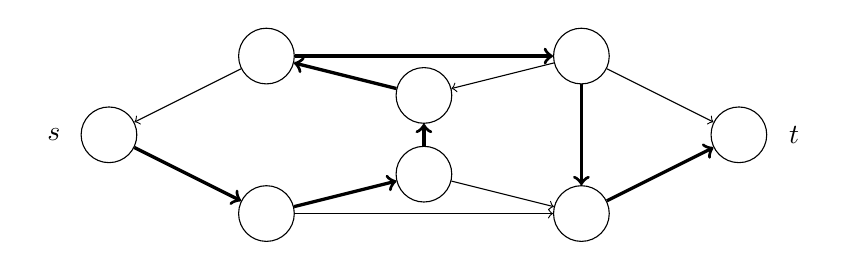
\begin{tikzpicture}
[inner sep=2.5mm]      
\path ( 0,1) node (0) [shape=circle,draw] {}
(2,2) node (1) [shape=circle,draw] {}
(2,0) node (2) [shape=circle,draw] {}
(4,1.5) node (3) [shape=circle,draw] {}
(4,0.5) node (4) [shape=circle,draw] {}
(6,2) node (5) [shape=circle,draw] {}
(6,0) node (6) [shape=circle,draw] {}
(8,1) node (7) [shape=circle,draw] {};
\path ( -0.7,1) node {$s$};
\path ( 8.7,1) node {$t$};
\draw [->] (1) -- (0);
\draw [->] (5) -- (3);
\draw [->] (5) -- (7);
\draw [->] (2) -- (6);
\draw [->] (4) -- (6);
\draw [->, very thick] (4) -- (3);
\draw [->, very thick] (0) -- (2);
\draw [->, very thick] (3) -- (1);
\draw [->, very thick] (1) -- (5);
\draw [->, very thick] (5) -- (6);
\draw [->, very thick] (2) -- (4);
\draw [->, very thick] (6) -- (7);
\end{tikzpicture}
\end{center}

  
\item $\text{HAMPATH}=\{\langle  G,s,t\rangle \mid G:$ directed,
a Hamiltonian path from $s$ to $t\}$
\item Brute-force

node 1 ... node $n$

0       1    0

check all paths
\item polynomial verification

for a path, in P time $\Rightarrow$ HAM or not

verification easier than determination

\end{itemize}\end{frame} \begin{frame}[allowframebreaks] \frametitle{Compositeness}
  \begin{itemize}
\item $x=pq, p, q > 1$
\item given $x$, difficult to find $p,q$

RSA
\item given $x,p,q$ easily verify $x=pq $ or not
\end{itemize}\end{frame} \begin{frame}[allowframebreaks] \frametitle{Not polynomial verifiable}
  \begin{itemize}
\item $\overline{HAMPATH}$: a graph does not have a Hamiltonian
path from $s$ to $t$

\item even if $\exists$ efficient way to determine

? how to verify

still need to check all paths

\end{itemize}\end{frame} \begin{frame}[allowframebreaks] \frametitle{Verifier}
  \begin{itemize}
\item algorithm V: a verifier of a language A
  \begin{equation*}
    A=\{w\mid
V \mbox{ accepts } 
\langle  w,c\rangle  
\mbox{ for some strings } c\}
  \end{equation*}
Ex: $\langle  w,c\rangle  = \langle  x,p\rangle $ (one divisor is enough)

$\langle  w,c\rangle  = \langle  \langle  G,s,t\rangle , \mbox{a path from $s$ to $t$}\rangle $
\item polynomial verifier: polynomial time of $|w|$
\item we measure time on $|w|$ only

\item A: polynomially verifiable if 
$\exists$ a polynomial verifier
\item $c$: ``certificate''

$|c|$ should be in polynomial of $|w|$

Otherwise, reading $|c|$ already non-polynomial
\end{itemize}\end{frame} \begin{frame}[allowframebreaks] \frametitle{NP}
  \begin{itemize}
\item languages have polynomial verifiers
\item $\Leftrightarrow$ decided by 
Nondeterministic Polynomial TM (proved later)

where the name comes from

Some use this as the definition

\item Note: NPTM: time by the longest branch

\end{itemize}\end{frame} \begin{frame}[allowframebreaks] \frametitle{NTM for HAMPATH}
  \begin{itemize}
\item list $p_1\cdots p_m$

nondeterministically determined
\item A tree with many lists
\item each list: check repetitions

check $s=p_1$; $t=p_m$

\item For $1 \ldots m-1, (p_i, p_{i+1})$ edge of $G$
\item work on each list: polynomial

repetitions: $O(m^2)$

$s=p_1, t = p_m: O(m)$

edge: $O(m^2)$

\end{itemize}\end{frame} \begin{frame}[allowframebreaks] \frametitle{NP: decided NPTM}

  \begin{itemize}
\item polynomial verifier $\Leftrightarrow$ P NTM

idea:

\item ``$\Rightarrow$'' NTM by guessing certificate

\item ``$\Leftarrow$'' using NTM's accepting branch as  certificate

\end{itemize}\end{frame} \begin{frame}[allowframebreaks] \frametitle{Proof}
  \begin{itemize}
\item ``$\Rightarrow$'': V: the verifier in time $O(n^k)$

$|c|\leq n^k$
\item An  NTM:
  \begin{enumerate}
  \item nondeterministically select $c$
  \item run V on $\langle  w,c\rangle $
  \end{enumerate}
i.e. run $c$ in parallel, each polynomial
\item ``$\Leftarrow$'' a V with input $\langle  w,c\rangle $

$c$: list of one branch

NPTM: each branch polynomial

note: in the definition of V, requires only ``some c''


\end{itemize}\end{frame} \begin{frame}[allowframebreaks] \frametitle{NP}
  \begin{itemize}
\item Def:

NTIME$(t(n)) = \{L\mid L
\text{ decided by } O(t(n))
\text{ nondeterministic TM}\}$
\item NP = $\cup_k \text{NTIME}(n^k)$

\end{itemize}\end{frame} \begin{frame}[allowframebreaks] \frametitle{Prove a problem is NP ?}
  \begin{itemize}
\item every branch polynomial time
\end{itemize}\end{frame} \begin{frame}[allowframebreaks] \frametitle{Clique Problem}
  \begin{itemize}
\item clique: a fully subgraph connected

Fig 7.23

clique: means a small group of people

\item $k$-clique: $k$ \# nodes
\item problem: whether $G$ has a clique of given \# nodes
\end{itemize}\end{frame} \begin{frame}[allowframebreaks] \frametitle{CLIQUE is NP}
  \begin{itemize}
\item try to identify some certificate

clique is $c$
\item $V$: input $\langle  \langle  G,k\rangle ,c\rangle $

$\langle  G,k\rangle $ given and some claims $c$ is a $k$-clique. Verify it
  \begin{enumerate}
  \item \# nodes of $c$ is $k$ ?
  \item $c$ fully connected and edges in $G$
  \end{enumerate}
  \item $V$ is polynomial
  \item Easily think from NPTM

(omitted here)



\end{itemize}\end{frame} \begin{frame}[allowframebreaks] \frametitle{SUBSET-SUM}
  \begin{itemize}
\item Given $x_1, \ldots, x_k$
\item ? sum of a subset $=t$
\item Formally
  \begin{eqnarray*}
&&    \{\langle  s,t\rangle 
\mid s=\{x_1, \ldots, x_k\}
\mbox{ and }
\exists \\
&&\qquad \qquad \{y_1, \ldots, y_l\}
\subset \{x_1, \ldots, x_k\},
\sum y_i =t\}
\end{eqnarray*}

\item Example

$\langle  \{4,11,16,21,27\},25\rangle $ OK
as 4+21=25
\item Note: allow repetition here

$\langle  \{4,11,11,16,21,27\},25\rangle $ 
 \end{itemize}\end{frame} \begin{frame}[allowframebreaks] \frametitle{SUBSET-SUM NP}
  \begin{itemize}
 \item V: input $\langle  \langle  s,t\rangle ,c\rangle $
  \begin{enumerate}
  \item check if $\sum c_i=t$
  \item check if all $c_i \in S$
  \end{enumerate}
\item length of $c <$  length of $s$
\end{itemize}\end{frame} \begin{frame}[allowframebreaks] \frametitle{Complements}
  \begin{itemize}
\item $\overline{CLIQUE}$,
$\overline{SUBSET-SUM}$ ? NP

not that easy

\item coNP: languages whose complements are NP

?coNP = NP, not known
\end{itemize}\end{frame} \begin{frame}[allowframebreaks] \frametitle{P vs. NP}
  \begin{itemize}
\item Roughly

P: problems decided quickly

NP: problems verified quickly
\item ? P= NP

one of the greatest unsolved problems

Fig 7.26

\item most believe P $\neq $ NP
\end{itemize}\end{frame} \begin{frame}[allowframebreaks] \frametitle{NP-completeness}
  \begin{itemize}
\item Problems in NP: related

\item For certain NP problems:

Polynomial algorithm of one NP $\Rightarrow$ P = NP



\item These probelsm: called NP-complete
\item To prove $P \neq NP$: only need to focus on
NP-complete problems
\item To prove $P=NP$: need only polynomial algorithms
for an NP-complete problem
\end{itemize}
\end{frame}
\end{document}
